\documentclass{scalatekids-article}
\usepackage[italian]{babel}
\begin{document}
\lfoot{Piano Di Qualifica 2.0.0}
\newgeometry{top=3.5cm}
\begin{titlepage}
  \begin{center}
    \begin{center}
      
\includegraphics[width=10cm]{sklogo.png}
    \end{center}
    \vspace{1cm}
    \begin{Huge}
      \begin{center}
        \textbf{Piano di Qualifica}
      \end{center}
    \end{Huge}
    \vspace{11pt}
    \bgroup
    \def\arraystretch{1.3}
    \begin{tabular}{r|l}
      \multicolumn{2}{c}{\textbf{Informazioni sul documento}} \\
      \hline
      \setbox0=\hbox{0.0.1\unskip}\ifdim\wd0=0pt
      \\
      \else
      \textbf{Versione} & 2.0.0\\
      \fi
      \textbf{Redazione} & \multiLineCell[t]{Francesco Agostini\\Giacomo  Vanin\\Marco Boseggia}\\
      \textbf{Verifica} & \multiLineCell[t]{Andrea Giacomo Baldan\\Michael Munaro}\\
      \textbf{Approvazione} & \multiLineCell[t]{Alberto De Agostini}\\
      \textbf{Uso} & Esterno\\
      \textbf{Lista di Distribuzione} & \multiLineCell[t]{ScalateKids\\Prof. Tullio Vardanega\\Prof. Riccardo Cardin}\\
    \end{tabular}
    \egroup
    \vspace{22pt}
  \end{center}
\end{titlepage}
\restoregeometry
\clearpage
\pagenumbering{Roman}
\setcounter{page}{1}
\begin{flushleft}
  \vspace{0cm}
         {\large\bfseries Diario delle modifiche \par}
\end{flushleft}
\vspace{0cm}
\begin{center}
  \begin{tabular}{| l | l | l | l | p{5cm} |}
    \hline
    Versione & Autore & Ruolo & Data & Descrizione \\
    \hline
    1.2.0 & Davide Trevisan & Verificatore & 2016-04-02 & Verifica sezioni test di validazione e di integrazione\\
    \hline
    1.1.1 & Alberto De Agostini & Progettista & 2016-04-01 & Stesura sezioni test di validazione e di integrazione\\
    \hline
    1.1.0 & Marco Boseggia & Verificatore & 2016-02-26 & Verifica sezioni 2.8.1 e sottosezioni\\
    \hline
    1.0.2 & Francesco Agostini & Analista & 2016-02-24 & Stesura sezione 2.8.1 e sottosezioni\\
    \hline
    1.0.1 & Francesco Agostini & Analista & 2016-02-19 & Ristesura sezione 2.2 in seguito alle correzioni del docente\\
    \hline
    1.0.0 & Alberto De Agostini & Responsabile & 2016-01-21 & Approvazione documento\\
    \hline
    0.6.0 & Andrea Giacomo Baldan & Verificatore & 2016-01-21 & Verifica sezione Resoconto attività di Verifica\\
    \hline
    0.5.2 & Francesco Agostini & Analista & 2016-01-21 & Stesura sezione Resoconto attività di Verifica\\
    \hline
    0.5.1 & Francesco Agostini & Analista & 2016-01-20 & Creazione scheletro sezione Resoconto attività di Verifica\\
    \hline
    0.5.0 & Michael Munaro & Verificatore & 2016-01-20 & Verifica Pianificazione dei test\\
    \hline
    0.4.2 & Marco Boseggia & Analista & 2016-01-18 & Integrazione sezione Pianificazione dei test\\
    \hline
    0.4.1 & Giacomo Vanin & Analista & 2016-01-17 & Stesura sezione Pianificazione dei test\\
    \hline
    0.4.0 & Michael Munaro & Verificatore & 2016-01-16 & Verifica Correzioni sezione Standard di Qualità\\
    \hline
    0.3.1 & Giacomo Vanin & Analista & 2016-01-16 & Correzioni sezione Standard di Qualità\\
    \hline
    0.3.0 & Andrea Giacomo Baldan & Verificatore & 2016-01-12 & Verifica sezione Standard di Qualità\\
    \hline
    0.2.1 & Marco Boseggia & Analista & 2016-01-09 & Stesura sezione Standard di Qualità\\
    \hline
    0.2.0 & Michael Munaro & Verificatore & 2016-01-07 & Verifica Correzione effettuata\\
    \hline
    0.1.1 & Giacomo Vanin & Analista & 2016-01-08 & Correzione sezione Gestione amministrativa della revisione\\
    \hline
    0.1.0 & Andrea Giacomo Baldan & Verificatore & 2016-01-05 & Verifica capitoli stesi in precedenza\\
    \hline
    0.0.3 & Giacomo Vanin & Analista & 2016-01-04 & Stesura sezione Gestione amministrativa della revisione\\
    \hline
    0.0.2 & Francesco Agostini & Analista & 2016-01-02 & Stesura sezione Visione generale della strategia di verifica\\
    \hline
    0.0.1 & Andrea Giacomo Baldan & Amministratore & 2015-12-16 & Creazione scheletro del documento\\
    \hline
  \end{tabular}
\end{center}
\tableofcontents
\newpage
\pagenumbering{arabic}
\section{Sommario}
\subsection{Scopo del documento}
Il seguente documento ha lo scopo di delineare le strategie che il gruppo \textit{ScalateKids} ha deciso di adottare per garantire degli obiettivi qualitativi da applicare ai processi sfruttati per lo sviluppo del progetto \textbf{ActorBase}. Per raggiungere tali obiettivi è necessario svolgere un'\gloss{attività} di verifica continua in modo da rilevare e correggere errori o malfunzionamenti minimizzando lo spreco di risorse.
\prodPurpose
\glossExpl
\subsection{Riferimenti}
\subsubsection{Normativi}
\begin{itemize}
\item\textbf{Capitolato d'appalto C1:} \textit{Actorbase: a NoSQL DB based on the Actor model;}\\
  \url{http://www.math.unipd.it/~tullio/IS-1/2015/Progetto/C1.pdf}
\item\textbf{Norme di Progetto:} \href{run:../Interni/NormeDiProgetto\_v2.0.0.pdf}{Norme di Progetto v2.0.0.}
\end{itemize}
\subsubsection{Informativi}
\begin{itemize}
\item\textbf{Piano di Progetto:} \href{run:./PianoDiProgetto\_v2.0.0.pdf}{Piano di Progetto v2.0.0}
\item\textbf{Dispense fornite dall'insegnamento Ingegneria del Software mod. A:}\\
  \url{http://www.math.unipd.it/~tullio/IS-1/2015/}
\item\textbf{Standard \gloss{ISO}/\gloss{IEC} 15504:}\\
\url{https://en.wikipedia.org/wiki/ISO/IEC_15504}
\item\textbf{Standard \gloss{ISO}/\gloss{IEC} 9126:}\\
\url{https://it.wikipedia.org/wiki/ISO/IEC_9126}
\item\textbf{\gloss{Ciclo di Deming}:}\\
\url{https://en.wikipedia.org/wiki/PDCA}
\end{itemize}
\newpage
\section{Visione generale della strategia di verifica}
\subsection{Definizione obiettivi}
\subsubsection{Qualità di processo}
Per perseguire la qualità del prodotto è necessario garantire la qualità dei processi attuati per la sua creazione. Per raggiungere questo scopo i \textit{Verificatori} con approvazione del \textit{Responsabile} hanno trovato utile adottare lo standard \gloss{ISO}/\gloss{IEC} 15504\footnote[1]{Per approfondimenti consultare la sezione \ref{sec:ISO/IEC15504}.} denominato SPICE (Software Process Improvement and Capability dEtermination). Il \gloss{ciclo di Deming}\footnote[2]{Per approfondimenti consultare la sezione \ref{PDCA}.} (noto anche come ciclo \gloss{PDCA}) definisce un metodo di controllo costante sui processi, consentendone un miglioramento continuo. Questo miglioramento consente ai processi di aumentare il livello di maturità nella scala data dallo standard \gloss{ISO}/\gloss{IEC} 15504.
\subsubsection{Qualità di prodotto}
I \textit{Verificatori} con approvazione del \textit{Responsabile} hanno deciso di seguire lo standard \gloss{ISO}/\gloss{IEC} 9126\footnote[3]{Per approfondimenti consultare la sezione \ref{sec:ISO/IEC9126}.} che ha lo scopo di delineare delle metriche per la misurazione della qualità di prodotto. Questa è fondamentale per garantire che il prodotto \gloss{software} finale funzioni correttamente e rispetti degli obiettivi di qualità prefissati.
\subsection{Procedure di controllo di qualità di processo}
Per applicare correttamente il \gloss{PDCA} è necessario che le seguenti condizioni siano soddisfatte:
\begin{itemize}
\item{Ci sia una pianificazione accurata dei processi;}
\item{Le risorse siano divise in maniera chiara nella pianificazione;}
\item{I processi siano controllati.}
\end{itemize}
La pianificazione descritta nel \href{run:./PianoDiProgetto\_v2.0.0.pdf}{Piano di Progetto v2.0.0} è stata fatta cercando di soddisfare queste condizioni.\\
Per avere una misurazione oggettiva e quantitativa della qualità su ogni processo sono state stabilite delle metriche di valutazione descritte nella sezione \ref{sec:metricheProcesso}. Tali misurazioni saranno effettuate periodicamente ogni venti giorni.\\
L'insieme di queste condizioni e metriche consente l'utilizzo del \gloss{PDCA} garantendo un miglioramento continuo della qualità di ogni processo e, di conseguenza, del prodotto finale.
\subsection{Procedure di controllo di qualità di prodotto}
Il controllo di qualità del prodotto si suddividerà in tre parti:
\begin{itemize}
\item{Attuazione di tecniche di analisi statica e dinamica descritte nella sezione \ref{sec:TecnicheDiAnalisi};}
\item{Verifica costante dell'output di ogni \gloss{attività}, i cui risultati verranno riportati nell'appendice \ref{sec:resAttivitaVerifica};}
\item{Validazione, ovvero la conferma che il prodotto risponda correttamente ai requisiti attesi.}
\end{itemize}
Per avere una misurazione oggettiva e quantitativa della qualità su ogni prodotto sono state stabilite delle metriche di valutazione per documenti e software descritte nelle sezioni, rispettivamente, \ref{sec:metricheDocumenti} e \ref{sec:metricheSW}. Queste misurazioni saranno effettuate ogniqualvolta viene prodotto un file, sia esso un documento o un file di codice.\\
\subsection{Organizzazione}
Per garantire la qualità del prodotto finale verranno effettuate \gloss{attività} di verifica su ogni processo attuato. I controlli su ogni processo avranno come obiettivo garantire la qualità sia del processo stesso sia dell'eventuale prodotto da esso ricavato.\\
Ogni fase descritta in \href{run:./PianoDiProgetto\_v2.0.0.pdf}{Piano di Progetto v2.0.0} necessita di \gloss{attività} di verifica diverse a causa della differenza natura del loro output. Di seguito sono elencate le strategie di verifica usate per ciascuna fase:
\begin{itemize}
\item\textbf{Analisi:} durante questa fase verrà verificato che ogni documento creato sia conforme a quanto descritto nel documento \href{run:../Interni/NormeDiProgetto\_v2.0.0.pdf}{Norme di Progetto v2.0.0}, inoltre sarà necessario controllare che ogni requisito sia associato a un caso d'uso e viceversa;
\item\textbf{Progettazione:} durante questa fase l'\gloss{attività} di verifica si concentrerà sul processo incrementale dei documenti prodotti in fase di Analisi e sui processi attuati per l'\gloss{attività} di progettazione assicurandosi che ogni documento e ogni processo sia conforme a quanto descritto nelle \href{run:../Interni/NormeDiProgetto\_v2.0.0.pdf}{Norme di Progetto v2.0.0};
\item\textbf{Codifica:} durante questa fase l'\gloss{attività} di verifica si concentrerà sul processo incrementale dei documenti prodotti in fase di Analisi e sui processi attuati per l'\gloss{attività} di codifica assicurandosi che ogni documento e ogni processo sia conforme a quanto descritto nelle \href{run:../Interni/NormeDiProgetto\_v2.0.0.pdf}{Norme di Progetto v2.0.0}.
\item\textbf{Verifica e Validazione:} durante questa fase l'\gloss{attività} di verifica continuerà ad essere sul processo incrementale dei documenti prodotti nelle precedenti fasi. Inoltre sarà effettuata una corposa \gloss{attività} di verifica per il collaudo del prodotto.
\end{itemize}
In ogni documento viene inoltre tenuto un diario delle modifiche per permettere di mantenere uno storico delle \gloss{attività} svolte su di esso e delle responsabilità per ogni \gloss{attività}.
\subsection{Pianificazione strategica e temporale}
L'\gloss{attività} di redazione di ogni documento sarà sempre anticipata da uno studio sulla struttura e sui contenuti del documento interessato. In questo modo si riduce la possibilità di errori concettuali e il tempo effettivo di scrittura del documento viene ridotto.\\
Il processo di verifica deve essere ben organizzato e pianificato per rispettare le scadenze fissate nel \href{run:./PianoDiProgetto\_v2.0.0.pdf}{Piano di Progetto v2.0.0}.\\
L'attività di verifica segue le metodologie descritte nelle \href{run:../Interni/NormeDiProgetto\_v2.0.0.pdf}{Norme di Progetto v2.0.0}. Esse sono state pensate in maniera tale da consentire l'individuazione e la correzione degli errori il più presto possibile evitando che si diffondano.
\subsection{Responsabilità}
Per organizzare al meglio il lavoro e in particolare le \gloss{attività} di verifica e validazione vengono assegnati questi compiti ai soli \textit{Verificatori} e al \textit{Responsabile}. Inoltre le \gloss{attività} di verifica non potranno essere svolte da un membro che ha partecipato allo sviluppo di tale sezione per garantire assenza di conflitto di interessi.
\subsection{Tecniche di analisi}
\label{sec:TecnicheDiAnalisi}
\subsubsection{Analisi statica}
L'analisi statica è una tecnica atta a trovare errori e anomalie. Questa tecnica è applicabile sia alla documentazione sia al \gloss{codice}.
\paragraph{Walkthrough}
\label{sec:walkthrough}Come descritto nelle \textit{\href{run:../Interni/NormeDiProgetto_v2.0.0.pdf}{Norme di Progetto v2.0.0}} verrà effettuata la tecnica walkthrough nelle fasi iniziali di ogni \gloss{attività} per passare il prima possibile ad \gloss{attività} di \textit{Inspection} (paragrafo seguente).
\paragraph{Inspection}
\label{sec:inspection}Successivamente all'\gloss{attività} di \ref{sec:walkthrough} {Walthrough} verrà fatta \gloss{attività} di inspection (seguendo \textit{Norme di Progetto} (paragrafo precedente)) rispetto alla lista di controllo ottenuta in precedenza.
\subsubsection{Analisi dinamica}
L'analisi dinamica si applica solo al prodotto software e serve a trovare errori o difetti nell'implementazione.\\I test effettuati devono essere \textit{ripetibili}; questa caratteristica è fondamentale poiché un test deve produrre sempre lo stesso risultato dato un input in un ambiente per trovare errori.
\paragraph{Test di unità}
Test per verificare ogni unità del software prodotto. Per unità si intende la più piccola quantità di software che è utile verificare singolarmente.\\L'obiettivo di questi test è trovare ed eliminare possibili errori creati dai \textit{programmatori}.
\paragraph{Test di integrazione}
Test per verificare che l'integrazione tra due o più unità software funzionino correttamente.\\In mancanza di unità questi test possono essere svolti tramite la creazione di una o più componenti fittizie che simulano il comportamento delle unità con cui l'unità creata deve interfacciarsi.
\paragraph{Test di sistema}
Test per verificare la totale copertura dei requisiti software emersi in fase di \textit{Analisi dei Requisiti}. Questi test verificano la totalità del prodotto software al suo raggiungimento di una versione definitiva.
\paragraph{Test di regressione}
Test da effettuare per verificare che una modifica del software non pregiudichi il funzionamento del sistema o di altre parti del prodotto prima correttamente funzionanti.\\
Questa \gloss{attività} dev'essere svolta tenendo conto del tracciamento dei requisiti per individuare i giusti test di unità, di integrazione e di sistema che possono essere influenzati dalle modifiche effettuate.\\
\paragraph{Test di accettazione}
Questo corrisponde al collaudo vero e proprio del software da svolgersi col \textit{Proponente}.
\subsection{Metriche di valutazione}
Per rendere quantificabile il processo di verifica verranno usate delle metriche elencate sotto. Soltanto due tipi di \gloss{range} saranno accettati:
\begin{itemize}
  \item \textbf{Ottimale}: contiene i valori che si deve cercare di ottenere, valori al di fuori di questo \gloss{range} dovranno essere verificati e, se necessario, discussi dal gruppo;
  \item \textbf{Accettazione}: valori per avere un'accettazione del prodotto.
\end{itemize}
\subsubsection{Metriche per i processi}
\label{sec:metricheProcesso}
Per garantire un monitoraggio e un controllo dei processi è stato scelto di utilizzare un indice sui costi e un indice temporale.
\paragraph{Budget Variance (BV)}
Questo indice indica se alla data corrente si è in linea con i costi preventivati.\\ Per calcolare questo indice basta moltiplicare le ore di lavoro pianificate per i rispettivi costi e sottrarle alla moltiplicazione tra le ore preventivate per i rispettivi costi.
Se \gloss{BV} è $\geq$ 0 significa che le spese sostenute sono minori rispetto ai costi preventivati.\\
\textbf{Range accettabili:}
\begin{itemize}
  \item \gloss{Range} ottimale: $\geq$ 0;
  \item \gloss{Range} di accettazione: $\geq$ -600. %TODO percentuale di accettazione
\end{itemize}
\paragraph{Schedule Variance (SV)}
Questo indice indica se alla data corrente si è in anticipo o in ritardo rispetto alla pianificazione temporale.\\ Per calcolare questo indice basta sottrarre le ore effettive alle ore pianificate. Il risultato indica una quantità di ore lavoro.\\
Se \gloss{SV} è $\geq$ 0 significa che si è in anticipo rispetto a quanto pianificato.\\
\textbf{Range accettabili:}
\begin{itemize}
  \item \gloss{Range} ottimale: $\geq$ 0;
  \item \gloss{Range} di accettazione: $\geq$ -40.
\end{itemize}

\subsubsection{Metriche per i documenti}
\label{sec:metricheDocumenti}
Per la stesura dei documenti è stato scelto di utilizzare un \textit{indice di leggibilità} per la lingua italiana.
\paragraph{Indice Gulpease}
\label{par:metricheGulpease}
Questo indice indica il grado di leggibilità di un documento.\\L'indice di Gulpease prende in considerazione principalmente tre variabili:
\begin{itemize}
\item Numero delle frasi;
\item Numero delle lettere;
\item Numero delle parole.
\end{itemize}
La formula applicata per calcolare il suddetto indice è:
\begin{center}
\begin{equation}
  89 + \cfrac{300 * (numero delle frasi) - 10 * (numero delle lettere)}{numero delle parole}
\end{equation}
\end{center}
Lo script applicato su un documento produrrà in output un valore intero compreso tra zero e cento, in particolare i significati sono i seguenti:
\begin{itemize}
  \item Indice inferiore a 80 rappresenta un documento difficile da leggere per persone con una licenza di scuola elementare;
  \item Indice inferiore a 60 rappresenta un documento difficile da leggere per persone con una licenza di scuola media inferiore;
  \item Indice inferiore a 40 rappresenta un documento difficile da leggere per persone con una licenza di diploma superiore;
\end{itemize}
\textbf{Range accettabili:}
\begin{itemize}
  \item \gloss{Range} ottimale: 60 - 100;
  \item \gloss{Range} di accettazione: 45 - 60.
\end{itemize}
\subsubsection{Metriche per il software}
\label{sec:metricheSW}
Per perseguire una buona qualità software sono state pensate diverse metriche di valutazione descritte nei prossimi paragrafi. Tuttavia questa sezione è una sezione che potrà subire cambiamenti durante le prossime revisioni.
\paragraph{Linee di codice per linee di commento}
Applicato su un file produrrà un valore in output che rappresenta la percentuale di righe di commento rispetto alle linee di \gloss{codice}.\\
\textbf{Range accettabili:}
\begin{itemize}
  \item \gloss{Range} ottimale: 30 - 40\%;
  \item \gloss{Range} di accettazione: 20 - 30\%.
\end{itemize}
\subsubsection{Copertura del codice}
La copertura del \gloss{codice} indica il numero di istruzioni che vengono eseguite durante i test rispetto alla totalità delle istruzioni. Per avere una minor possibilità di presenza di errori nel \gloss{codice} si dovrà avere una percentuale il più alta possibile di istruzioni testate.\\Tuttavia metodi molto semplici che non necessitano testing andranno a influire negativamente in questo ambito.\\
\textbf{Range accettabili:}
\begin{itemize}
  \item \gloss{Range} ottimale: 60 - 100\%;
  \item \gloss{Range} di accettazione: 40 - 60\%.
\end{itemize}
\subsubsection{Numero di attributi per classe}
Un numero troppo elevato di attributi in una classe potrebbe indicare il non soddisfacimento del principio di \textit{\gloss{single responsability}}. Questo potrebbe significare la necessità di una divisione in più classi relazionate tra loro per dividere le diverse funzionalità o un possibile errore di progettazione.\\
\textbf{Range accettabili:}
\begin{itemize}
  \item \gloss{Range} ottimale: 3 - 6;
  \item \gloss{Range} di accettazione: 0 - 12.
\end{itemize}
\subsubsection{Numero di parametri per metodo}
Un numero troppo elevato di parametri in un metodo potrebbe indicare il non soddisfacimento del principio di \textit{\gloss{single responsability}}. Questo potrebbe significare la necessità di una divisione in sotto metodi per dividere le diverse funzionalità o un possibile errore di progettazione.\\
\textbf{Range accettabili:}
\begin{itemize}
  \item Range ottimale: 0 - 4;
  \item Range di accettazione: 4 - 8.
\end{itemize}
\subsubsection{Complessità ciclomatica}
La complessità ciclomatica è usata per misurare la complessità di parti di \gloss{codice} come funzioni, metodi, classi o moduli.\\
Questa è calcolata attraverso un grafo di controllo del flusso del programma.\\La complessità ciclomatica di una sezione di \gloss{codice} è il numero di cammini linearmente indipendenti attraverso il \gloss{codice} sorgente. Per esempio, se il \gloss{codice} sorgente non contiene punti decisionali come IF o cicli FOR, allora la complessità sarà 1, poiché esiste un solo cammino nel sorgente (e quindi nel grafo). Se il \gloss{codice} ha un singolo IF contenente una singola condizione, allora ci saranno due cammini possibili: il primo se l'IF viene valutato a TRUE e un secondo se l'IF viene valutato a FALSE.\\
\textbf{Range accettabili:}
\begin{itemize}
  \item \gloss{Range} ottimale: 0 - 10;
  \item \gloss{Range} di accettazione: 10 - 15.
\end{itemize}
\subsubsection{Livelli di annidamento}
Indica il numero di livelli di annidamento di funzioni e metodi. Un valore alto di questo indice implica un livello di complessità molto elevato, aumentando la probabilità di commettere errori.\\
\textbf{Range accettabili:}
\begin{itemize}
  \item \gloss{Range} ottimale: 1 - 4;
  \item \gloss{Range} di accettazione 5 - 8.
\end{itemize}
\newpage
\appendix
\section{Standard di qualità}
\subsection{Standard ISO/IEC 15504}
\label{sec:ISO/IEC15504}
Lo standard \gloss{ISO}/\gloss{IEC} 15504 definisce un metodo per controllare continuamente la qualità di ogni processo. Questo metodo sfrutta un modello denominato SPY (Software Process Assessment and Improvement) per la valutazione di processo.\\
%TODO immagine SPY
Questo standard fornisce i seguenti nove attributi di qualità di processo:
\begin{itemize}
  \item{\textbf{Process performance:} il processo riesce a trasformare input identificabili in output identificabili.;}
  \item{\textbf{Performance management:} Il processo viene attuato e controllato seguendo una pianificazione che garantisca il raggiungimento degli obiettivi;}
  \item{\textbf{Work product management:} Il processo viene attuato e controllato seguendo una pianificazione che garantisca risultati documentati e verificati;}
  \item{\textbf{Process definition:} Il processo viene attuato seguendo standard di processo per garantire i risultati;}
  \item{\textbf{Process resource:} Il processo ha risorse adeguate per la sua attuazione;}
  \item{\textbf{Process measurement:} I risultati raggiunti e le misure rilevate durante l'attuazione di un processo sono stati usati per assicurarsi che tale processo supporti il raggiungimento di specifici obiettivi;}
  \item{\textbf{Process control:} Ogni processo è controllato attraverso la raccolta, analisi ed utilizzo delle misure di prodotto e di processo rilevate, per migliorare, eventualmente, le sue modalità di attuazione;}
  \item{\textbf{Process change:} Le modifiche alla definizione, gestione e attuazione di ogni processo sono controllate;}
  \item{\textbf{Continuous improvement:} Le modifiche ad ogni processo sono identificate ed implementate per assicurare il continuo miglioramento nel raggiungimento degli obiettivi rilevanti per l'organizzazione.}
\end{itemize}
Questi attributi vengono utilizzati per suddividere la maturità di un processo nei seguenti sei livelli:
\begin{itemize}
  \item{\textbf{Livello 0 - Incompleto:} Il processo non raggiunge i suoi obiettivi;}
  \item{\textbf{Livello 1 - Attuato:} Il processo raggiunge i suoi obiettivi ma non è controllato. Il raggiungimento di questo livello è dimostrato dal possesso dell'attributo di \textit{Process Performance};}
  \item{\textbf{Livello 2 - Gestito:} Il processo è attuato, pianificato, tracciato, verificato e migliorato sulla base di obiettivi ben definiti. Il raggiungimento di questo livello è dimostrato dal possesso dell'attributo di \textit{Performance management} e \textit{Work product management};}
  \item{\textbf{Livello 3 - Definito:} Il processo è attuato, pianificato e controllato su procedure basate sui principi del software engineering. Il raggiungimento di questo livello è dimostrato dal possesso dell'attributo di \textit{Process definition} e \textit{Process resource};}
  \item{\textbf{Livello 4 - Predicibile:} Il processo è stabilizzato ed è attuato all’interno di definiti limiti riguardo i risultati attesi, le performance e le risorse impiegate. Il raggiungimento di questo livello è dimostrato dal possesso dell'attributo di \textit{Performance measurement} e \textit{Process control};}
  \item{\textbf{Livello 5 - Ottimizzante:} Il processo è predicibile ed in grado di adattarsi per raggiungere obiettivi specifici e rilevanti per la organizzazione. Il raggiungimento di questo livello è dimostrato dal possesso dell'attributo di \textit{Process change} e \textit{Continuous improvement}.}
\end{itemize}
\begin{figure}[H]
  \begin{center}
    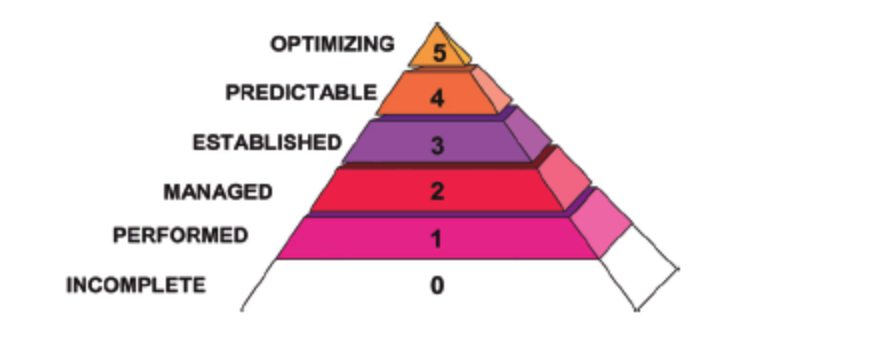
\includegraphics[width=0.6\textwidth, keepaspectratio]{ISO15504.png}
    \caption{Visione piramidale dei sei livelli di maturità di processo.}
  \end{center}
\end{figure}
Infine per stabilire in che livello si trovi un processo ci sono quattro livelli di possesso per ogni attributo:
\begin{itemize}
  \item{\textbf{N:} Non posseduto;}
  \item{\textbf{P:} Parzialmente posseduto;}
  \item{\textbf{L:} Largamente posseduto;}
  \item{\textbf{F:} Pienamente (Fully) posseduto.}
\end{itemize}
\subsection{Ciclo di Deming}
\label{PDCA}
Il \gloss{ciclo di Deming}, anche chiamato \gloss{PDCA}, è un modello che consente il miglioramento continuo dei processi. Si suddivide nelle seguenti quattro \gloss{attività}:
\begin{itemize}
  \item{\textbf{Plan:} \gloss{attività} di pianificazione di \gloss{attività}, risorse, scadenze e responsabilità;}
  \item{\textbf{Do:} \gloss{attività} di esecuzione delle \gloss{attività} pianificate;}
  \item{\textbf{Check:} \gloss{attività} di verifica dei risultati dell'\gloss{attività} di esecuzione, questi risultati verranno poi confrontati con i risultati pianificati nella fase di pianificazione;}
  \item{\textbf{Act:} \gloss{attività} di messa in pratica del miglioramento dei processi sfruttando i risultati dell'\gloss{attività} di verifica per trovare e modificare gli aspetti critici.}
\end{itemize}
\begin{figure}[H]
  \begin{center}
    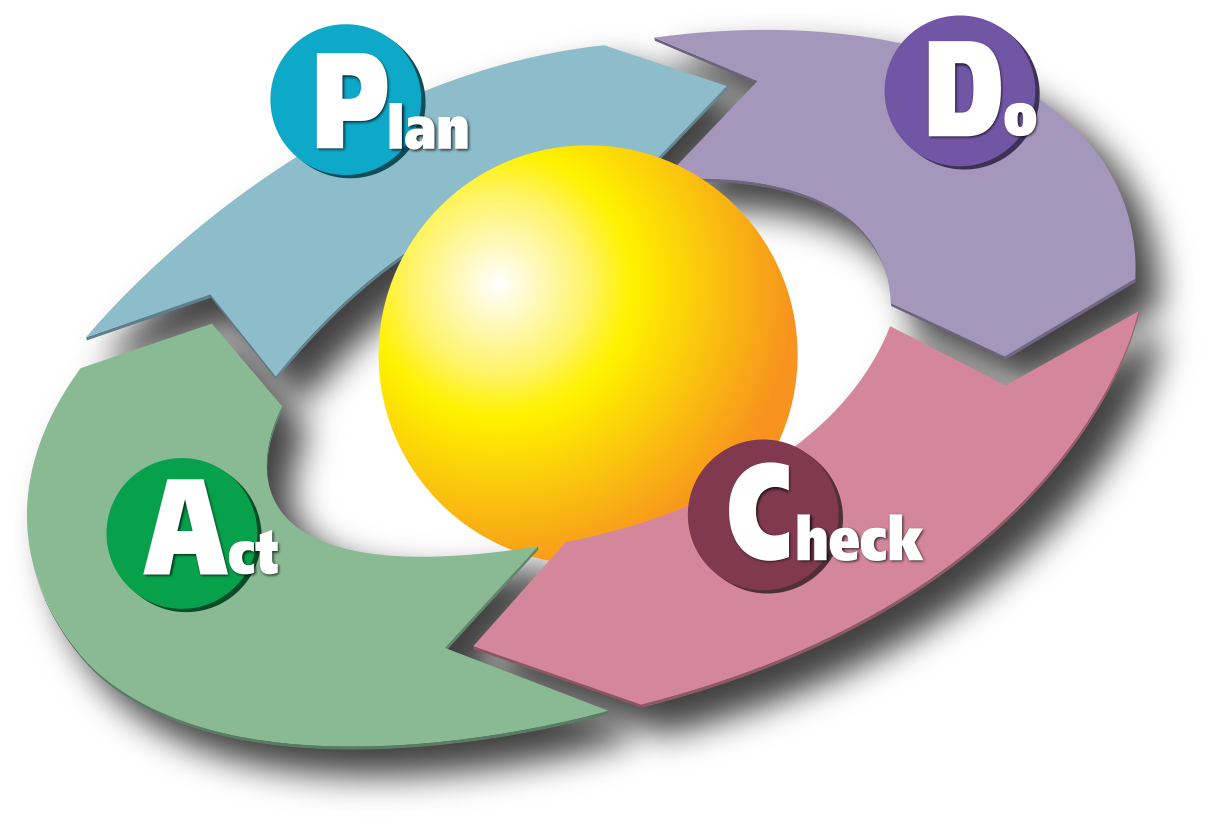
\includegraphics[width=0.5\textwidth, keepaspectratio]{PDCA.png}
    \caption{Ciclo di Deming}
  \end{center}
\end{figure}
\subsection{Standard ISO/IEC 9126}
\label{sec:ISO/IEC9126}
Lo standard \gloss{ISO}/\gloss{IEC} 9126 definisce un modello per migliorare l'organizzazione e i processi, avendo come conseguenza il miglioramento della qualità del prodotto finale. I criteri qualitativi sono divisi in tre \gloss{macro} aree:
\begin{itemize}
  \item{\textbf{Qualità interna:} è la qualità del prodotto software vista dall'interno. Si riferisce alla valutazione del \gloss{codice} sorgente e dell'architettura prima che il prodotto sia ultimato;}
  \item{\textbf{Qualità esterna:} è la qualità del prodotto software vista dall'esterno. Si riferisce al risultato dei test condotti sul prodotto ultimato in un ambiente di prova;}
  \item{\textbf{Qualità in uso:} è la qualità del prodotto vista dall'utilizzatore finale del prodotto. Si riferisce alla qualità dopo il rilascio dell'applicazione.}
\end{itemize}
Non potendo testare la qualità in uso nell'ambito di questo progetto si è scelto di concentrarsi sulla qualità interna ed esterna. Queste qualità nello standard \gloss{ISO}/\gloss{IEC} 9126 sono ulteriormente suddivise in sei categorie:
\begin{figure}[H]
  \begin{center}
    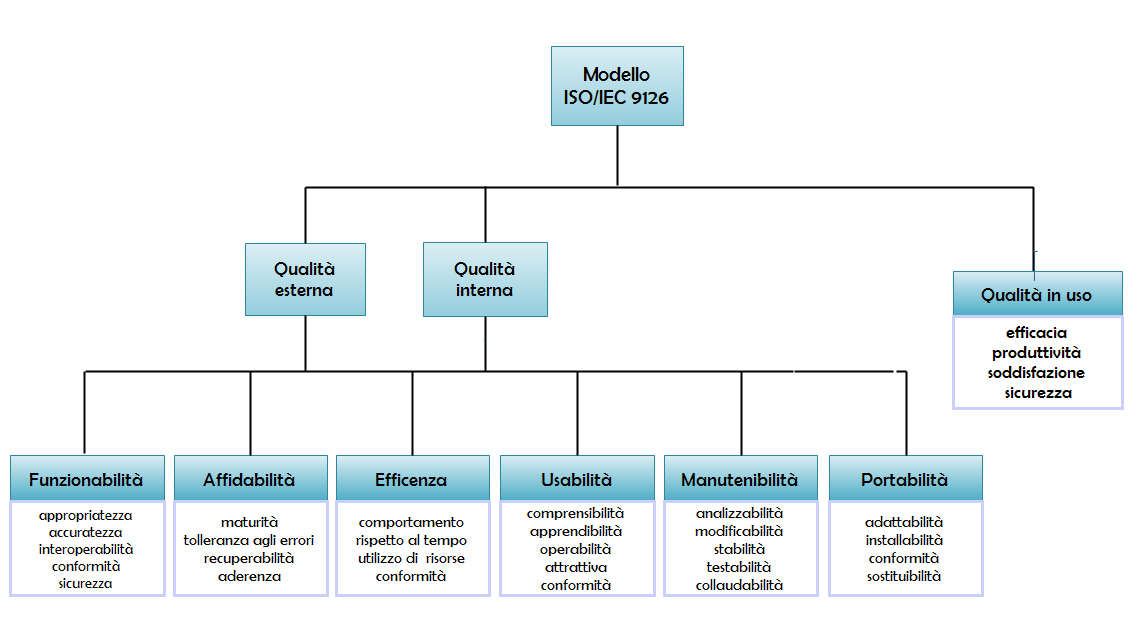
\includegraphics[width=0.9\textwidth, keepaspectratio]{Modello_ISO-IEC_9126.png}
    \caption{Modello dello standard ISO/IEC 9126}
  \end{center}
\end{figure}
\begin{itemize}
  \item{\textbf{Funzionalità:} capacità del prodotto di fornire funzioni che soddisfino esigenze stabilite. Questa categoria si suddivide in:}
    \begin{itemize}
      \item{\textbf{Appropriatezza:} capacità del prodotto di fornire un appropriato insieme di funzioni che rispondano a determinati requisiti;}
      \item{\textbf{Accuratezza:} capacità del prodotto di fornire dei risultati corretti o con precisione concordata;}
      \item{\textbf{Interoperabilità:} capacità del prodotto di interagire con uno o più sistemi esterni;}
      \item{\textbf{Conformità:} capacità del prodotto di aderire a standard del settore di applicazione;}
      \item{\textbf{Sicurezza:} capacità del prodotto di proteggere i dati, ad esempio negando l'accesso a utenti non autorizzati.}
    \end{itemize}
  \item{\textbf{Affidabilità:} capacità del prodotto di mantenere uno specificato livello di prestazioni durante un determinato periodo. Questa categoria si suddivide in:}
    \begin{itemize}
      \item{\textbf{Maturità:} capacità del prodotto di evitare che si verifichino risultati non corretti a causa di errori nel software;}
      \item{\textbf{Tolleranza agli errori:} capacità del prodotto di mantenere uno specificato livello di prestazioni anche in presenza di errori nel software o di uso scorretto del prodotto;}
      \item{\textbf{Recuperabilità:} capacità del prodotto di ristabilire un livello adeguato di prestazioni in seguito a un malfunzionamento;}
      \item{\textbf{Aderenza:} capacità del prodotto di a standard riguardanti l'affidabilità.}
    \end{itemize}
  \item{\textbf{Efficienza:} capacità del prodotto di fornire prestazioni appropriate in relazione alle risorse usate. Questa categoria si suddivide in:}
    \begin{itemize}
      \item{\textbf{Comportamento rispetto al tempo:} capacità del prodotto di fornire i risultati in tempi adeguati;}
      \item{\textbf{Utilizzo delle risorse:} capacità del prodotto di utilizzare le risorse in modo adeguato;}
      \item{\textbf{Conformità:} capacità del prodotto di aderire a standard sull'efficienza.}
    \end{itemize}
  \item{\textbf{Usabilità:} capacità del prodotto di essere capito e usato dall'utente. Questa categoria si suddivide in:}
    \begin{itemize}
      \item{\textbf{Comprensibilità:} facilità di comprensione del prodotto;}
      \item{\textbf{Apprendibilità:} capacità di ridurre l'impegno richiesto all'utente per imparare come usare correttamente il prodotto finale;}
      \item{\textbf{Operabilità:} capacità del prodotto di fare in modo che gli utenti riescano a farne uso per i propri scopi;}
      \item{\textbf{Attrattiva:} capacità del prodotto di essere piacevole per l'utente;}
      \item{\textbf{Conformità:} capacità del prodotto di aderire a standard sull'usabilità.}
    \end{itemize}
  \item{\textbf{Manutenibilità:} capacità del prodotto di essere modificato e migliorato. Questa categoria si suddivide in:}
    \begin{itemize}
      \item{\textbf{Analizzabilità:} facilità di analisi del \gloss{codice} per la localizzazione di errori;}
      \item{\textbf{Modificabilità:} capacità del prodotto di permettere la sostituzione di componenti per implementare una determinata modifica;}
      \item{\textbf{Stabilità:} capacità del prodotto di evitare errori derivanti da modifiche errate;}
      \item{\textbf{Testabilità:} capacità del prodotto di essere facilmente testato rispetto alle modifiche apportate.}
    \end{itemize}
  \item{\textbf{Portabilità:} capacità del prodotto di essere trasportato in un altro ambiente di lavoro. Questa categoria si suddivide in:}
    \begin{itemize}
      \item{\textbf{Adattabilità:} capacità del prodotto di essere adattato per ambienti operativi diversi senza modifiche diverse da quelle fornite;}
      \item{\textbf{Installabilità:} capacità del prodotto di essere installato in specifici ambienti;}
      \item{\textbf{Conformità:} capacità del prodotto di aderire a standard sulla portabilità;}
      \item{\textbf{Sostituibilità:} capacità del prodotto di essere utilizzato al posto di un altro software per svolgere gli stessi compiti.}
    \end{itemize}
\end{itemize}
\newpage
\section{Resoconto attività di verifica}
\label{sec:resAttivitaVerifica}
\subsection{Attività di Analisi}
\subsubsection{Documenti}
Nella tabella di seguito sono riportati i valori degli indici di Gulpease per ogni documento prodotto durante l'\gloss{attività} di Analisi. L'esito della verifica dipenderà dal valore di questo indice come descritto nella sezione \ref{par:metricheGulpease}.
\begin{center}
  \begin{tabular}{| c | c | c |}
    \hline
    Documento & Valore indice & Esito\\
    \hline
    \textit{Studio di Fattibilità v1.0.0} & 54.18 & Superato\\
    \textit{Norme di Progetto v1.0.0} & 52.04 & Superato\\
    \textit{Piano di Progetto v1.0.0} & 54.87 & Superato\\
    \textit{Piano di Qualifica v1.0.0} & 52.82 & Superato\\
    \textit{Analisi dei Requisiti v1.0.0} & 68.06 & Superato\\
    \textit{Glossario v1.0.0} & 47.42 & Superato\\
    \hline
  \end{tabular}
\end{center}
\subsection{Attività di Progettazione}
\subsubsection{Documenti}
Nella tabella di seguito sono riportati i valori degli indici di Gulpease per ogni documento prodotto durante l'\gloss{attività} di Progettazione. L'esito della verifica dipenderà dal valore di questo indice come descritto nella sezione \ref{par:metricheGulpease}.
\begin{center}
  \begin{tabular}{| c | c | c |}
    \hline
    Documento & Valore indice & Esito\\
    \hline
    \textit{Studio di Fattibilità v2.0.0} &  & Superato\\
    \textit{Norme di Progetto v2.0.0} &  & Superato\\
    \textit{Piano di Progetto v2.0.0} &  & Superato\\
    \textit{Piano di Qualifica v2.0.0} &  & Superato\\
    \textit{Analisi dei Requisiti v2.0.0} &  & Superato\\
    \textit{Glossario v2.0.0} &  & Superato\\
    \hline
  \end{tabular}
\end{center}
\newpage
\section{Pianificazione dei test}

Di seguito sono descritti i test di sistema. In futuro questa sezione verrà aggiornata con i test di integrazione e di unità.

\subsection{Test di sistema}

I test di sistema permettono di verificare il comportamento del sistema rispetto ai requisiti descritti nell'\href{run:./AnalisiDeiRequisiti\_v2.0.0.pdf}{Analisi dei requisiti v2.0.0}.\\
La tabella seguente descrive i test dei requisiti ritenuti meritevoli di verifica. \\
La colonna "Stato" nella tabella è lasciata vuota in quanto i test saranno effettuati successivamente.
\begin{center}
  \begin{longtable}[H]{| l | p{10cm} | l | l |}
    \hline
    Test & Descrizione & Stato & Requisito\\
    \hline
    TS.OBF1 & Viene verificato che il sistema dovrà fornire la possibilità di distribuire il carico all'interno di un cluster scalabile & & OBF1\\
    \hline
    TS.OBF1.1 & Viene verificato che il \gloss{cluster} dovrà fornire la possibilità di connettersi ai singoli \gloss{nodi} del \gloss{cluster} & & OBF1.1\\
    \hline
    TS.OBF1.1.1 & Viene verificato che il singolo \gloss{nodo} dovrà fornire un server per ricevere comandi dall'esterno e inviare risposte & & OBF1.1.1\\
    \hline
    TS.OBF1.1.10.1 & Viene verificato che il sistema ad attori dovrà permettere di autenticarsi dall'esterno mediante interazioni tra \gloss{Clientactor}, \gloss{Mainactor}, \gloss{Storefinder} e \gloss{Userkeeper} & & OBF1.1.10.1\\
    \hline
    TS.OBF1.1.10.2.1 & Viene verificato che il sistema ad attori dovrà permettere di creare \gloss{collezioni} mediante l'interazione tra \gloss{Clientactor}, \gloss{Mainactor}, \gloss{Storefinder}, \gloss{Storekeeper} e \gloss{Userkeeper} & & OBF1.1.10.2.1\\
    \hline
    TS.OBF1.1.10.2.2 & Viene verificato che il sistema ad attori dovrà permettere di visualizzare una lista delle \gloss{collezioni} mediante l'interazione con \gloss{Clientactor} & & OBF1.1.10.2.2\\
    \hline
    TS.OBF1.1.10.2.3 & Viene verificato che il sistema ad attori dovrà permettere di modificare il nome delle \gloss{collezioni} mediante l'interazione tra \gloss{Clientactor}, \gloss{Mainactor}, \gloss{Storefinder} e \gloss{Userkeeper} & & OBF1.1.10.2.3\\
    \hline
    TS.OBF1.1.10.2.4 & Viene verificato che il sistema ad attori dovrà permettere di cancellare \gloss{collezioni} mediante l'interazione tra \gloss{Clientactor}, \gloss{Mainactor}, \gloss{Storefinder}, \gloss{Storekeeper}, \gloss{Userkeeper} e \gloss{Ninja} & & OBF1.1.10.2.4\\
    \hline
    TS.OBF1.1.10.2.5 & Viene verificato che il sistema ad attori dovrà permettere di aggiungere collaboratori a \gloss{collezioni} & & OBF1.1.10.2.5\\
    \hline
    TS.OBF1.1.10.2.6 & Viene verificato che il sistema ad attori dovrà permettere di rimuovere collaboratori da \gloss{collezioni} mediante l'interazione tra \gloss{Clientactor}, \gloss{Mainactor}, \gloss{Storefinder}, \gloss{Storekeeper}, \gloss{Userkeeper} e \gloss{Ninja} & & OBF1.1.10.2.6\\
    \hline
    TS.OBF1.1.10.2.7 & Viene verificato che il sistema ad attori dovrà permettere di esportare \gloss{collezioni} mediante l'interazione tra \gloss{Clientactor}, \gloss{Mainactor}, \gloss{Storefinder}, \gloss{Storekeeper}, \gloss{Userkeeper} e \gloss{Ninja} & & OBF1.1.10.2.7\\
    \hline
    TS.OBF1.1.10.3.1 & Viene verificato che il sistema ad attori dovrà permettere di inserire \gloss{item} mediante l'interazione tra \gloss{Clientactor}, \gloss{Mainactor}, \gloss{Storefinder}, \gloss{Storekeeper}, \gloss{Ninja} e \gloss{Manager} & & OBF1.1.10.3.1\\
    \hline
    TS.OBF1.1.10.3.2 & Viene verificato che il sistema ad attori dovrà permettere di creare una \gloss{collezione} nel caso di inserimento \gloss{item} a \gloss{collezione} inesistente mediante interazioni tra \gloss{Clientactor}, \gloss{Mainactor} e \gloss{Userkeeper} & & OBF1.1.10.3.2\\
    \hline
    TS.OBF1.1.10.3.3 & Viene verificato che il sistema ad attori dovrà inviare un messaggio d'errore verso l'esterno nel caso in cui la chiave dell'\gloss{item} da inserire senza sovrascrittura sia già presente, mediante interazioni tra \gloss{Clientactor}, \gloss{Mainactor}, \gloss{Storefinder} e \gloss{Storekeeper} & & OBF1.1.10.3.3\\
    \hline
    TS.OBF1.1.10.3.4 & Viene verificato che il sistema ad attori dovrà permettere di cancellare \gloss{item} da \gloss{collezioni} mediante interazioni tra \gloss{Clientactor}, \gloss{Main}, \gloss{Storefinder}, \gloss{Storekeeper} e \gloss{Ninja} & & OBF1.1.10.3.4\\
    \hline
    TS.OBF1.1.10.3.5 & Viene verificato che il sistema ad attori dovrà inviare un messaggio d'errore verso l'esterno nel caso in cui il nome della \gloss{collezione} a cui inserire nuovi \gloss{item} sia inesistente, mediante interazioni tra \gloss{Clientactor} ed esterno & & OBF1.1.10.3.5\\
    \hline
    TS.OBF1.1.10.4 & Viene verificato che il sistema ad attori dovrà permettere di ricercare \gloss{item} tra \gloss{collezioni} mediante interazioni tra \gloss{Clientactor}, \gloss{Main}, \gloss{Storefinder} e \gloss{Storekeeper} & & OBF1.1.10.4\\
    \hline
    TS.OBF1.1.10.5 & Viene verificato che il sistema ad attori dovrà permettere di modificare la password utente di uno \gloss{username} mediante interazioni tra \gloss{Clientactor}, \gloss{Main}, \gloss{Storefinder}, \gloss{Userkeeper} & & OBF1.1.10.5\\
    \hline
    TS.OBF1.1.10.6 & Viene verificato che il sistema ad attori dovrà permettere la disconnessione di client esterni mediante interazioni con \gloss{Clientactor} & & OBF1.1.10.6\\
    \hline
    TS.OBF1.1.10.7.1 & Viene verificato che il sistema ad attori dovrà permettere di aggiungere nuovi utenti all'interno del \gloss{database} mediante interazioni tra \gloss{Clientactor},\gloss{Main}, \gloss{Storefinder} e \gloss{Userkeeper} & & OBF1.1.10.7.1\\
    \hline
    TS.OBF1.1.10.7.2 & Viene verificato che il sistema ad attori dovrà permettere la rimozione di un utente dal \gloss{database} mediante interazioni tra \gloss{Clientactor}, \gloss{Main}, \gloss{Storefinder} & & OBF1.1.10.7.2\\
    \hline
    TS.OBF1.1.10.7.3 & Viene verificato che il sistema ad attori dovrà permettere di effettuare un reset della password di un utente mediante interazioni tra \gloss{Clientactor}, \gloss{Main}, \gloss{Storefinder}, \gloss{Userkeeper} & & OBF1.1.10.7.3\\
    \hline
    TS.OBF2 & Viene verificato che il sistema dovrà fornire una \gloss{console} per inviare comandi al server (CLI) & & OBF2\\
    \hline
    TS.OBF2.1 & Viene verificato che il sistema dovrà fornire un Domain Specific Language per comunicare con il \gloss{database} & & OBF2.1\\
    \hline
    TS.OBF2.1.1 & Viene verificato che il DSL dovrà fornire un comando per effettuare l'autenticazione utilizzabile mediante CLI & & OBF2.1.1\\
    \hline
    TS.OBF2.1.2.1 & Viene verificato che il DSL dovrà fornire un comando per la creazione di una nuova \gloss{collezione} utilizzabile mediante CLI & & OBF2.1.2.1\\
    \hline
    TS.OBF2.1.2.2 & Viene verificato che il DSL dovrà fornire un comando per elencare i nomi delle \gloss{collezioni} presenti all’interno del \gloss{database} utilizzabile mediante CLI & & OBF2.1.2.2\\
    \hline
    TS.OBF2.1.2.3 & Viene verificato che il DSL dovrà fornire un comando per cancellare una o più \gloss{collezioni} utilizzabile mediante CLI & & OBF2.1.2.3\\
    \hline
    TS.OBF2.1.2.4 & Viene verificato che il DSL dovrà fornire un comando per modificare il nome delle {collezioni} utilizzabile mediante CLI & & OBF2.1.2.4\\
    \hline
    TS.OBF2.1.2.5 & Viene verificato che il DSL dovrà fornire un comando per aggiungere \gloss{collaboratori} ad una \gloss{collezione} del sistema utilizzabile mediante CLI & & OBF2.1.2.5\\
    \hline
    TS.OBF2.1.2.6 & Viene verificato che il DSL dovrà fornire un comando per rimuovere un \gloss{collaboratore} da una \gloss{collezione} del sistema utilizzabile mediante CLI & & OBF2.1.2.6\\
    \hline
    TS.OBF2.1.2.7 & Viene verificato che il DSL dovrà fornire un comando per l'esportazione di \gloss{collezioni} su file \gloss{JSON} utilizzabile mediante CLI & & OBF2.1.2.7\\
    \hline
    TS.OBF2.1.3.1 & Viene verificato che il DSL dovrà fornire un comando per inserire un nuovo \gloss{item} utilizzabile mediante CLI & & OBF2.1.3.1\\
    \hline
    TS.OBF2.1.3.1.1 & Viene verificato che il DSL dovrà fornire un comando per inserire un \gloss{item} specificandone gli attributi da CLI & & OBF2.1.3.1.1\\
    \hline
    TS.DEF2.1.3.1.2 & Viene verificato che il DSL dovrà fornire un comando per inserire nuovi \gloss{item} da file \gloss{JSON} utilizzabile mediante CLI & & DEF2.1.3.1.2\\
    \hline
    TS.DEF2.1.4 & Viene verificato che il DSL dovrà fornire un comando per richiedere aiuto generale sul sistema utilizzabile mediante CLI & & DEF2.1.4\\
    \hline
    TS.DEF2.1.5 & Viene verificato che il DSL dovrà fornire un comando per richiedere aiuto sull'utilizzo di uno specifico comando del sistema utilizzabile mediante CLI  & & DEF2.1.5\\
    \hline
    TS.OBF2.1.6 & Viene verificato che il DSL dovrà fornire un comando per permettere di effettuare una ricerca su una o più \gloss{collezioni} all'interno del sistema; utilizzabile mediante CLI & & OBF2.1.6\\
    \hline
    TS.OBF2.1.7 & Viene verificato che il DSL dovrà fornire un comando per la modifica della propria password utilizzabile mediante CLI & & OBF2.1.7\\
    \hline
    TS.OBF2.1.8 & Viene verificato che il DSL dovrà fornire un comando per effettuare il logout dal sistema utilizzabile mediante CLI & & OBF2.1.8\\
    \hline
    TS.OBF2.1.9.1 & Viene verificato che il DSL dovrà fornire un comando per l'aggiunta di un nuovo utente all'interno del sistema utilizzabile mediante CLI & & OBF2.1.9.1\\
    \hline
    TS.OBF2.1.9.2 & Viene verificato che il DSL dovrà fornire un comando per la rimozione di un utente dal sistema & & OBF2.1.9.2\\
    \hline
    TS.OBF2.1.9.3 & Viene verificato che il DSL dovrà fornire un comando per effettuare il reset della password di un utente alla password standard & & OBF2.1.9.3\\
    \hline
    TS.DEF3 & Viene verificato che dovrà essere fornito un \gloss{driver} \gloss{Scala} per interfacciarsi con il \gloss{database} & & DEF3\\
    \hline
    TS.DEF3.1 & Viene verificato che il \gloss{driver} dovrà permettere di effettuare l'autenticazione all'interno del sistema. & & DEF3.1\\
    \hline
    TS.DEF3.2.1 & Viene verificato che il \gloss{driver} dovrà permettere un la creazione di una nuova \gloss{collezione} & & DEF3.2.1\\
    \hline
    TS.DEF3.2.2 & Viene verificato che il \gloss{driver} dovrà permettere di elencare i nomi delle \gloss{collezioni} presenti all’interno del \gloss{database} & & DEF3.2.2\\
    \hline
    TS.DEF3.2.3 & Viene verificato che il \gloss{driver} dovrà permettere di cancellare una o più \gloss{collezioni}  & & DEF3.2.3\\
    \hline
    TS.DEF3.2.4 & Viene verificato che il \gloss{driver} dovrà permettere di modificare il nome delle {collezioni} & & DEF3.2.4\\
    \hline
    TS.DEF3.2.5 & Viene verificato che il \gloss{driver} dovrà permettere di aggiungere \gloss{collaboratori} ad una \gloss{collezione} del sistema & & DEF3.2.5\\
    \hline
    TS.DEF3.2.6 & Viene verificato che il \gloss{driver} dovrà permettere di rimuovere un \gloss{collaboratore} da una \gloss{collezione} del sistema & & DEF3.2.6\\
    \hline
    TS.DEF3.2.7 & Viene verificato che il \gloss{driver} dovrà permettere di esportare \gloss{collezioni} su file \gloss{JSON} & & DEF3.2.7\\
    \hline
    TS.DEF3.3.1 & Viene verificato che il \gloss{driver} dovrà permettere di inserire un nuovo \gloss{item} & & DEF3.3.1\\
    \hline
    TS.DEF3.3.1.1 & Viene verificato che il \gloss{driver} dovrà permettere di inserire un nuovo \gloss{item} specificandone gli attributi & & DEF3.3.1.1\\
    \hline
    TS.DEF3.3.1.2 & Viene verificato che il \gloss{driver} dovrà permettere di inserire nuovi \gloss{item} da file \gloss{JSON} & & DEF3.3.1.2\\
    \hline
    TS.DEF3.3.2 & Viene verificato che il \gloss{driver} dovrà permettere di cancellare uno o più \gloss{item} dal sistema & & DEF3.3.2\\
    \hline
    TS.DEF3.4 & Viene verificato che il \gloss{driver} dovrà permettere di effettuare ricerche su una o più \gloss{collezioni} all'interno del sistema & & DEF3.4\\
    \hline
    TS.DEF3.5 & Viene verificato che il \gloss{driver} dovrà permettere di effettuare il logout dal sistema & & DEF3.5\\
    \hline
    TS.DEF3.6.1 & Viene verificato che il \gloss{driver} dovrà permettere a utenti amministratori di aggiungere un nuovo utente al sistema & & DEF3.6.1\\
    \hline
    TS.DEF3.6.2 & Viene verificato che il \gloss{driver} dovrà permettere a utenti amministratori di rimuovere un utente dal sistema & & DEF3.6.2\\
    \hline
    TS.DEF3.6.3 & Viene verificato che il \gloss{driver} dovrà permettere a utenti amministratori di effettuare il reset della password ad un utente all'interno del sistema & & DEF3.6.3\\
    \hline
    TS.DEF3.7 & Viene verificato che il \gloss{driver} dovrà permettere di modificare la propria password & & DEF3.7\\
    \hline
    TS.DEF3.8 & Viene verificato che il \gloss{Driver} dovrà strutturare i dati in output in maniera navigabile & & DEF3.8\\
    \hline
    TS.OBV4 & Viene verificato che il sistema dovrà funzionare in ambienti Ubuntu 14.04 o superiore & & OBV4\\
    \hline
    TS.OBV5 & Viene verificato che il sistema dovrà funzionare su \gloss{JVM} versione 8 & & OBV5\\
    \hline
    TS.OBV6 & Viene verificato che il sistema dovrà utilizzare la libreria Akka versione 2.4.2 & & OBV6\\
    \hline
    TS.OBV7 & Viene verificato che il sistema dovrà essere implementato utilizzando il linguaggio Scala versione 2.11 & & OBV7\\
    \hline
    TS.DEV8 & Viene verificato che il sistema dovrà funzionare in ambienti Windows 10 o superiori & & DEV8\\
    \hline
    TS.DEV9 & Viene verificato che il sistema dovrà funzionare su sistemi OSX El Capitan o superiori & & DEV9\\
    \hline
    TS.OBQ10 & Viene verificato che dovrà essere fornito un manuale utente redatto in lingua inglese & & OBQ10\\
    \hline
    TS.OBQ11 & Viene verificato che dovranno essere rispettate tutte le norme e le metriche sulla stesura del codice come riportato nelle \textit{Norme di Progetto} & & OBQ11\\
    \hline
    TS.OBQ12 & Viene verificato che dovrà essere prodotta documentazione in Scaladoc del prodotto & & OBQ12\\
    \hline
  \end{longtable}
\end{center}

\subsection{Test di integrazione}

I test di integrazione permettono di verificare la corretta integrazione ed il
corretto flusso dei dati all'interno del sistema, sia relazioni tra
\gloss{package} sia il funzionamento
di ogni singolo \gloss{package} di ogni componente.\\
L'approccio utilizzato è di tipo \gloss{bottom-up}, in questo modo è possibile
integrare prima le parti con minore dipendenza funzionale e, nel caso di
inserimento di parti difettose, è possibile retrocedere ad uno stato testato e
sicuro in maniera semplice. Il diagramma seguente non rispetta il formalismo
\gloss{UML} 2.0 ed è utilizzato per semplificare l'illustrazione della strategia
di integrazione:
\begin{figure}[H]
  \begin{center}
    \includegraphics[width=1.0\textwidth, keepaspectratio]{RP/AlberoIntegrazione.png}
    \caption{Diagramma informale della strategia di integrazione}
  \end{center}
\end{figure}

\subsubsection{Descrizione dei test di integrazione}

La colonna "Stato" nella tabella è lasciata vuota in quanto i test saranno effettuati successivamente.

\begin{longtable}[H]{| l | p{10cm} | l | l |}
  \hline
  Test & Descrizione & Componente & Stato\\
  \hline
  TI.actorbase & Test di integrazione finale per le componenti cli, driver e actorsystem & actorbase &\\
  \hline
  TI.cli & Test di integrazione finale per models, views e controllers & cli &\\
  \hline
  TI.models & Verifica della corretta esecuzione dei comandi mediante integrazione con componente driver & models &\\
  \hline
  TI.controllers & Verifica del parsing dei comandi e della corretta integrazione con models e views & controllers &\\
  \hline
  TI.views & Verifica del corretto funzionamento delle procedure di input e output & views &\\
  \hline
  TI.driver & Test di integrazione finale per client, actorbasedata e serializer & driver &\\
  \hline
  TI.client & Verifica della comunicazione tra client e server e corretto funzionamento dei comandi & client &\\
  \hline
  TI.serializer & Test di controllo sulla corretta esecuzione delle procedure di serializzazione e deserializzazione secondo il protocollo \gloss{RESP} & serializer &\\
  \hline
  TI.actorbasedata & Verifica della corretta integrazione con le componenti client e serializer & actorbasedata &\\
  \hline
  TI.actorsystem & Test di integrazione finale per tcpserver, storefinder, storekeeper, ninja, manager, userkeeper, main, clientactor, serialization, warehouseman & actorsystem &\\
  \hline
  TI.serialization & Verifica delle corrette procedure di serializzazione e deserializzazione secondo i protocolli specificati & serialization &\\
  \hline
  TI.tcpserver & Test di verifica del corretto funzionamento del server tcp & tcpserver &\\
  \hline
  TI.clientactor & Test di verifica del parsing dei comandi riecvuti dall'esterno e della corretta esecuzione dei messaggi & clientactor &\\
  \hline
  TI.main & Verifica della corretta esecuzioni dei messaggi dedicati & main &\\
  \hline
  TI.storefinder & Verifica della corretta esecuzioni dei messaggi dedicati & storefinder &\\
  \hline
  TI.storekeeper & Verifica della corretta esecuzioni dei messaggi dedicati & storekeeper &\\
  \hline
  TI.userkeeper & Verifica della corretta esecuzioni dei messaggi dedicati & userkeeper &\\
  \hline
  TI.manager & Verifica della corretta esecuzioni dei messaggi dedicati & manager &\\
  \hline
  TI.ninja & Verifica della corretta esecuzioni dei messaggi dedicati & ninja &\\
  \hline
  TI.warehouseman & Verifica della corretta esecuzioni dei messaggi dedicati & warehouseman &\\
  \hline
\end{longtable}

\subsubsection{Tracciamento componenti-test di integrazione}

\begin{longtable}[H]{| p{10cm} | l |}
  \hline
  Componente & Test\\
  \hline
  actorbase & TI.actorbase\\
  \hline
  actorbase::cli & TI.cli\\
  \hline
  actorbase::cli::models & TI.models\\
  \hline
  actorbase::cli::controllers & TI.controllers\\
  \hline
  actorbase::cli::views & TI.views\\
  \hline
  actorbase::driver & TI.driver\\
  \hline
  actorbase::driver::client & TI.client\\
  \hline
  actorbase::driver::serializer & TI.serializer\\
  \hline
  actorbase::driver::actorbasedata & TI.actorbasedata\\
  \hline
  actorbase::actorsystem & TI.actorsystem\\
  \hline
  actorbase::actorsystem::serialization & TI.serialization\\
  \hline
  actorbase::actorsystem::tcpserver & TI.tcpserver\\
  \hline
  actorbase::actorsystem::clientactor & TI.clientactor\\
  \hline
  actorbase::actorsystem::main & TI.main\\
  \hline
  actorbase::actorsystem::storefinder & TI.storefinder\\
  \hline
  actorbase::actorsystem::storekeeper & TI.storekeeper\\
  \hline
  actorbase::actorsystem::userkeeper & TI.userkeeper\\
  \hline
  actorbase::actorsystem::manager & TI.manager\\
  \hline
  actorbase::actorsystem::ninja & TI.ninja\\
  \hline
  actorbase::actorsystem::warehouseman & TI.warehouseman\\
  \hline
\end{longtable}

\subsection{Test di validazione}

I test di validazione servono all'accertamento che il prodotto realizzato sia conforme
alle attese.\\
Per ogni test vengono descritti i passi che un utente deve eseguire per testare i
requisiti ad esso associati.\\
Si noti che i seguenti test eccetto \hyperref[sec:TV1]{TV1}, \hyperref[sec:TV3]{TV3} e \hyperref[sec:TV4]{TV4} rappresentano le operazioni possibili 
sul database, per questo motivo tutti questi test saranno effettuabili sia 
tramite l'utilizzo della \gloss{CLI} sia tramite l'utilizzo del \gloss{Driver}.\\
Nei test di validazione in cui è previsto l'inserimento di parametri per 
l'esecuzione di una operazione sul database si è scelto di non descrivere 
dettagliatamente tutti i parametri da inserire poiché questa descrizione è 
già stata redatta nell'\href{run:../Esterni/AnalisiDeiRequisiti\_v2.0.0.pdf}{Analisi dei Requisiti 2.0.0}.\\

\subsubsection{Test TV1}
\label{sec:TV1}

L'utente intende aggiungere un nodo al \gloss{cluster}.\\
L'utente deve:
\begin{itemize}
\item Avviare il server actorbase (TV1.1);
\item Adattare il file di configurazione per potersi connettere al \gloss{cluster} (TV1.2);
\item Avviare actorbase sul nuovo nodo (TV1.3);
\item Verificare tramite console l'avvenuta connessione al \gloss{cluster} (TV1.4).
\end{itemize}

\subsubsection{Test TV2}

L'utente intende autenticarsi presso il sistema.\\
L'utente deve:
\begin{itemize}
\item Inserire il comando per effettuare l'autenticazione (TV2.1);
\item Inserire i parametri per effettuare l'autenticazione (TV2.2);
\item Verificare che l'autenticazione ha avuto successo controllando la 
risposta ricevuta dal server o eseguendo un comando 
disponibile solo ad utenti autenticati (TV2.3).
\end{itemize}

\subsubsection{Test TV3}
\label{sec:TV3}

L'utente vuole richiedere aiuto generale.\\
L'utente deve:
\begin{itemize}
\item Inserire il comando di aiuto generale attraverso l'uso della \gloss{CLI} (TV3.1);
\item Verificare che l'output della richiesta di aiuto è stato stampato in 
output sulla \gloss{CLI} (TV3.2).
\end{itemize}

\subsubsection{Test TV4}
\label{sec:TV4}

L'utente vuole richiedere aiuto specifico di un comando.\\
L'utente deve:
\begin{itemize}
\item Inserire il comando di aiuto attraverso l'uso della \gloss{CLI} (TV4.1);
\item Inserire il nome del comando di cui vuole ricevere informazioni (TV4.2);
\item Verificare che l'output della richiesta di aiuto è stato stampato in 
output sulla \gloss{CLI} (TV4.3).
\end{itemize}

\subsubsection{Test TV5}

L'utente vuole creare una \gloss{collezione}.\\
L'utente deve:
\begin{itemize}
\item Inserire il comando per la creazione \gloss{collezione} (TV5.1);
\item Inserire il nome della \gloss{collezione} da creare (TV5.2);
\item Verificare l'avvenuta creazione della \gloss{collezione} controllando la 
risposta ricevuta dal server o usando il comando di visualizzazione 
lista delle collezioni (TV5.3).
\end{itemize}

\subsubsection{Test TV6}

L'utente vuole visualizzare la lista delle \gloss{collezioni}.\\
L'utente deve:
\begin{itemize}
\item Inserire il comando per la visualizzazione lista delle \gloss{collezioni} (TV6.1);
\item Verificare l'avvenuta esecuzione del comando controllando la risposta ricevuta dal server (TV6.2).
\end{itemize}

\subsubsection{Test TV7}

L'utente vuole modificare nome ad una propria \gloss{collezione}.\\
L'utente deve:
\begin{itemize}
\item Inserire il comando per la modifica nome \gloss{collezione} (TV7.1);
\item Inserire i parametri per cambiare il nome della \gloss{collezione} (TV7.2);
\item Verificare l'avvenuta esecuzione del comando controllando la risposta ricevuta dal server o usando il comando di visualizzazione lista delle collezioni (TV7.3).
\end{itemize}

\subsubsection{Test TV8}

L'utente vuole cancellare una \gloss{collezione}.\\
L'utente deve:
\begin{itemize}
\item Inserire il comando per la cancellazione \gloss{collezione} (TV8.1);
\item Inserire i parametri per cancellare la \gloss{collezione} (TV8.2);
\item Verificare l'avvenuta esecuzione del comando controllando la risposta ricevuta dal server o usando il comando di visualizzazione lista delle collezioni (TV8.3).
\end{itemize}

\subsubsection{Test TV9}

L'utente vuole aggiungere un collaboratore ad una \gloss{collezione}.\\
L'utente deve:
\begin{itemize}
\item Inserire il comando per 'aggiunta collaboratore a \gloss{collezione} (TV9.1);
\item Inserire i parametri per aggiungere il collaboratore alla  \gloss{collezione} (TV9.2);
\item Verificare l'avvenuta esecuzione del comando controllando la risposta ricevuta dal server (TV9.3).
\end{itemize}


\subsubsection{Test TV10}

L'utente vuole rimuovere un collaboratore da una \gloss{collezione}.\\
L'utente deve:
\begin{itemize}
\item Inserire il comando per la rimozione di un collaboratore da un \gloss{collezione} (TV10.1);
\item Inserire i parametri per rimuovere un collaboratore da una \gloss{collezione} (TV10.2);
\item Verificare l'avvenuta esecuzione del comando controllando la risposta ricevuta dal server (TV10.3).
\end{itemize}

\subsubsection{Test TV11}

L'utente vuole esportare una o più \gloss{collezioni} su file.\\
L'utente deve:
\begin{itemize}
\item Inserire il comando per l'esportazione di \gloss{collezioni} su file (TV11.1);
\item Inserire i parametri per esportare \gloss{collezioni} su file (TV11.2);
\item Verificare l'avvenuta esecuzione del comando controllando la risposta ricevuta dal server o controllando il file salvato su disco (TV11.3).
\end{itemize}

\subsubsection{Test TV12}

L'utente vuole inserire un \gloss{item}.\\
L'utente deve:
\begin{itemize}
\item Inserire il comando per l'inserimento di \gloss{item} (TV12.1);
\item Inserire i parametri per inserire l'\gloss{item} (TV12.2);
\item Verificare l'avvenuta esecuzione del comando controllando la risposta ricevuta dal server o usando il comando di ricerca sulla \gloss{collezione} giusta con la chiave appena usata (TV12.3).
\end{itemize}

\subsubsection{Test TV13}

L'utente vuole inserire un \gloss{item} importando da file.\\
L'utente deve:
\begin{itemize}
\item Inserire il comando per l'importazione di \gloss{item} da file (TV13.1);
\item Inserire i parametri per inserire gli \gloss{item} tramite importazione (TV13.2);
\item Verificare l'avvenuta esecuzione del comando controllando la risposta ricevuta dal server o usando il comando di ricerca sugli \gloss{item} appena inseriti (TV13.3).
\end{itemize}

\subsubsection{Test TV14}

L'utente vuole cancellare un \gloss{item}.\\
L'utente deve:
\begin{itemize}
\item Inserire il comando per la cancellazione di \gloss{item} (TV14.1);
\item Inserire i parametri per cancellare l'\gloss{item} (TV14.2);
\item Verificare l'avvenuta esecuzione del comando controllando la risposta ricevuta dal server o usando il comando di ricerca sulla \gloss{collezione} giusta con la chiave appena usata per effettuare la cancellazione (TV14.3).
\end{itemize}

\subsubsection{Test TV15}

L'utente vuole effettuare una ricerca di \gloss{item} su una o più \gloss{collezioni}.\\
L'utente deve:
\begin{itemize}
\item Inserire il comando per la ricerca di \gloss{item} (TV15.1);
\item Inserire i parametri per la ricerca di un \gloss{item} su una o più \gloss{collezioni} (TV15.2);
\item Verificare l'avvenuta esecuzione del comando controllando la risposta ricevuta dal server (TV15.3).
\end{itemize}

\subsubsection{Test TV16}

L'utente vuole visualizzare tutti gli \gloss{item} contenuti in una \gloss{collezione}.\\
L'utente deve:
\begin{itemize}
\item Inserire il comando per la ricerca di \gloss{item} (TV16.1);
\item Inserire i parametri per la ricerca di tutti gli \gloss{item} contenuti in una \gloss{collezione} (TV16.2);
\item Verificare l'avvenuta esecuzione del comando controllando la risposta ricevuta dal server (TV16.3).
\end{itemize}

\subsubsection{Test TV17}

L'utente vuole effettuare una ricerca di un \gloss{item} sull'intero database (secondo i suoi permessi come specificato nel documento \href{run:../Esterni/AnalisiDeiRequisiti\_v2.0.0.pdf}{Analisi dei Requisiti 2.0.0}).\\
L'utente deve:
\begin{itemize}
\item Inserire il comando per la ricerca di \gloss{item} (TV17.1);
\item Inserire i parametri per la ricerca di un \gloss{item} sull'intero database (TV17.2);
\item Verificare l'avvenuta esecuzione del comando controllando la risposta ricevuta dal server (TV17.3).
\end{itemize}

\subsubsection{Test TV18}

L'utente vuole visualizzare l'intero database (secondo i suoi permessi come specificato nel documento \href{run:../Esterni/AnalisiDeiRequisiti\_v2.0.0.pdf}{Analisi dei Requisiti 2.0.0}).\\
L'utente deve:
\begin{itemize}
\item Inserire il comando per la ricerca di \gloss{item} (TV18.1);
\item Inserire i parametri per la ricerca per l'intero database (TV18.2);
\item Verificare l'avvenuta esecuzione del comando controllando la risposta ricevuta dal server (TV18.3).
\end{itemize}

\subsubsection{Test TV19}

L'utente vuole effettuare modificare la propria password.\\
L'utente deve:
\begin{itemize}
\item Inserire il comando per la modifica password (TV19.1);
\item Inserire i parametri per la modifica password (TV19.2);
\item Verificare l'avvenuta esecuzione del comando controllando la risposta ricevuta dal server o effettuando una deautenticazione seguita da una autenticazione con la nuova password (TV19.3).
\end{itemize}

\subsubsection{Test TV20}

L'utente vuole effettuare deautenticazione dal server.\\
L'utente deve:
\begin{itemize}
\item Inserire il comando per effettuare il logout (TV20.1);
\item Verificare l'avvenuta esecuzione del comando controllando la risposta ricevuta dal server o eseguendo un comando disponibile solo ad utenti autenticati (che dovrà non essere disponibile) (TV20.2).
\end{itemize}

\subsubsection{Test TV21}

L'utente amministratore vuole aggiungere un utente al sistema.\\
L'utente deve:
\begin{itemize}
\item Inserire il comando per aggiungere un utente al sistema (TV21.1);
\item Inserire i parametri per l'aggiunta utente (TV21.2);
\item Verificare l'avvenuta esecuzione del comando controllando la risposta ricevuta dal server (TV21.3).
\end{itemize}

\subsubsection{Test TV22}

L'utente amministratore vuole rimuovere un utente dal sistema.\\
L'utente deve:
\begin{itemize}
\item Inserire il comando per la rimozione utente (TV22.1);
\item Inserire i parametri per la rimozione utente (TV22.2);
\item Verificare l'avvenuta esecuzione del comando controllando la risposta ricevuta dal server (TV22.3).
\end{itemize}

\subsubsection{Test TV23}

L'utente amministratore vuole effettuare un reset della password di un utente.\\
L'utente deve:
\begin{itemize}
\item Inserire il comando per effettuare il reset password (TV23.1);
\item Inserire i parametri per il reset password (TV23.2);
\item Verificare l'avvenuta esecuzione del comando controllando la risposta ricevuta dal server (TV23.3).
\end{itemize}

\listoffigures
\end{document}
